\documentclass[12pt,oneside,letterpaper,english]{article}
\usepackage[T1]{fontenc}
\usepackage[latin1]{inputenc}
\usepackage[margin=2.25cm,headheight=26pt,includeheadfoot]{geometry}
\usepackage[english]{babel}
\usepackage{listings}
\usepackage{color}
\usepackage{titlesec}
\usepackage{titling}
\usepackage[framed, numbered]{matlab-prettifier}
\usepackage{changepage}
\usepackage{amsmath}
\usepackage{hyperref}
\usepackage{enumitem}
\usepackage{graphicx}
\usepackage{float}
\usepackage{fancyhdr}
\usepackage{lastpage}
\usepackage{caption}
\usepackage{tocloft}
\usepackage{setspace}
\usepackage{multirow}
\usepackage{titling}
\usepackage{float}
\usepackage{comment}
\usepackage{booktabs}
\usepackage{indentfirst}
\usepackage{lscape}
\usepackage{booktabs,caption}
\usepackage[flushleft]{threeparttable}
\usepackage[english]{nomencl}
\usepackage{xcolor}
\usepackage{lipsum}
\usepackage{datetime2}
\usepackage{subcaption}	
\usepackage[table]{xcolor}
\usepackage{hyperref} % Already included somewhere
\usepackage{fontawesome5} % Load the FontAwesome5 package


\setlength{\parindent}{2em}
\lstset{language=Matlab,
style=Matlab-editor,
basicstyle=\normalsize\mlttfamily,
numbers=left,
numberstyle={\scriptsize\color{black}},	% size of the numbers
numbersep=0.5cm											
}
\newlist{steps}{enumerate}{1}
\setlist[steps, 1]{leftmargin=1.5cm,label = Step \arabic*:}
\renewcommand{\rmdefault}{ptm}

\begin{document}
\begin{titlepage}
	\begin{center}
		
		
\includegraphics[width=0.4\textwidth]{root/iit_logo.jpg}~\\[1cm]
		
		{\huge \bfseries{IC202P: Design Practicum Mid-Sem Report}}\\[1cm]
		{\huge \bfseries{Group 49}}\\[1cm]
		% Title
		\hrule
		\vspace{.5cm}
		{ \huge \bfseries Automated feature and defect analysis tool for semiconductors materials} % title of the report
		\vspace{.5cm}
		\hrule
		\vspace{1cm}
		
		\textsc{\textbf{\large Group Members}}\\
		\vspace{.5cm}
		\centering
		% add your name here
		
		\begin{tabular}{cc} \vspace{.2cm}
			B23247 & Anupam Prakash \\ \vspace{.15cm}
			B23210 & Keshav \\ \vspace{.15cm}
			B23215 & Mohit \\ \vspace{.15cm}
			B23323 & Martha Thrighun \\ \vspace{.15cm}
			B23289 & Ritika Verma \\
		\end{tabular}
		\vspace{.5cm}
		
		\textsc{\textbf{\large Faculty Mentors}}\\
		\vspace{.5cm}
		\centering
		Dr Neha Thakur, SMME \\ \vspace{.15cm} 
		Dr Parmod Kumar, SMME\\ 
		\vspace{4cm}
		
	\end{center}
\end{titlepage}

\newpage
\pagenumbering{roman}
\doublespacing
\renewcommand{\baselinestretch}{1}\normalsize
\hypersetup{hidelinks} % Removes red borders from ToC links
\tableofcontents
\renewcommand{\baselinestretch}{1}\normalsize

\newpage
\pagenumbering{arabic} 
\section{Introduction}
As semiconductor technology continues to advance, the demand for precise defect analysis and process control becomes more critical than ever. The performance and reliability of semiconductor devices are heavily influenced by the structural integrity of nanoscale features, where even minor variations can lead to electrical instabilities and yield loss. One of the key challenges in scanning electron microscope (SEM) image analysis is the presence of noise, artifacts, and process-induced roughness, which complicates defect detection and critical dimension measurements. \\

Traditional methods for analyzing these images rely on manual inspection or semi-automated software tools, which may lack the precision and efficiency required for large-scale semiconductor manufacturing. This underscores the need for an automated, accurate, and user-friendly tool that can extract meaningful roughness metrics from SEM images to enhance material characterization and quality control.\\  

In this project, we aim to develop a web-based tool that automates the analysis of SEM images by performing feature classification and roughness quantification. The tool will classify images into line-space patterns and contact-space patterns, enabling precise critical dimension (CD) measurements, as well as calculations of line-edge roughness (LER) and line-width roughness (LWR) for line-space patterns. Additionally, for contact-space images, it will compute the average diameter and ellipticity of features, ensuring a comprehensive analysis of various nanoscale structures. \\

\begin{itemize}
	\item \textbf{Line-Edge Roughness (LER):} Refers to the random deviations along the edges of a line in a semiconductor pattern. LER can impact device performance by introducing variability in transistor gate lengths, affecting threshold voltage stability and power consumption.
	
	\item \textbf{Line-Width Roughness (LWR):} Measures the fluctuations in the width of a patterned line, which can arise due to variations in lithography and etching processes. Excessive LWR can lead to unpredictable variations in circuit performance, especially in high-speed and low-power devices.  
	
	\item \textbf{Critical Dimension (CD) Measurement:} Determines the precise width or diameter of semiconductor features, a key metric in ensuring process consistency across wafers.
	
	\item \textbf{Power Spectral Density (PSD) Analysis:} Used to analyze spatial frequency components of roughness, helping to distinguish between systematic and stochastic roughness contributions in line patterns.
	
\end{itemize}
The tool will be designed to enhance efficiency and accuracy by integrating automated image processing algorithms, edge detection methods, and data visualization techniques. It will provide users with quantifiable roughness metrics, graphical representations such as PSD curves, and downloadable reports for further analysis. Additionally, the tool will be web-based, ensuring accessibility and ease of use without the need for specialized software installations.  \\

By addressing the limitations of existing metrology applications, our solution aims to streamline semiconductor defect analysis, improve yield predictions, and contribute to better process control in nanofabrication.\\

\section{List of potential solutions}
\subsection{Traditional Image Processing}
\textbf{Description:}\\
Traditional Image Processing use rule-based image processing techniques such as edge detection, thresholding, and morphological operations to identify defects in semiconductor materials. These methods analyze high-contrast images to detect anomalies based on predefined rules.\\

\textbf{Challenges:}
\begin{itemize}
\item 	Limited Adaptability: These systems work well for simple and well-defined defect types but struggle with complex or evolving defects.
\item	High Maintenance: Requires frequent parameter tuning when defect characteristics change.
\item	False Positives/Negatives: May fail to detect subtle defects or mistakenly classify normal patterns as defects.
\end{itemize}
\subsection{Deep Learning-Based Defect Detection (CNNs, ViTs, etc.)}
\textbf{Description:}\\
Deep learning-based models, particularly Convolutional Neural Networks (CNNs) and Vision Transformers (ViTs), are trained on large datasets of semiconductor images to automatically classify and localize defects. These models learn feature representations, making them more robust to variations in defect appearance.\\

\textbf{Challenges:}
\begin{itemize}
\item	Data Dependency: Requires a large, well-labeled dataset of SEM images for effective training.
\item	Computational Cost: Training and deploying deep learning models require high-end GPUs or TPUs, increasing infrastructure costs.
\item	Generalization Issues: Model performance may degrade when applied to new defect types not present in the training data.

\end{itemize}

\subsection{Unsupervised Anomaly Detection (Autoencoders, GANs, etc.)}
\textbf{Description:}\\
Instead of requiring labeled data, unsupervised learning methods like Autoencoders and Generative Adversarial Networks (GANs) learn the normal distribution of defect-free semiconductor images. Any deviation from this normality is flagged as an anomaly.\\

\textbf{Challenges:}
\begin{itemize}
	\item Subtle Defects: Some minor defects may not be distinguishable from natural variations, leading to misclassification.
	\item Model Sensitivity: Small environmental variations (e.g., noise in SEM images) may trigger false alarms.
	\item	Interpretability: Hard to explain why a specific region was classified as defective.
\end{itemize}

\subsection{Hybrid AI Approaches (Combination of CNNs + Rule-Based Methods)}
\textbf{Description:}\\
This approach combines deep learning-based feature extraction with traditional machine vision rules. CNNs detect complex defect patterns, while rule-based methods refine detection for well-understood defect types.\\

\textbf{Challenges:}
\begin{itemize}
	\item Integration Complexity: Requires expertise in both deep learning and classical computer vision.
	\item Computational Overhead: Hybrid models can be resource-intensive.
	\item Scalability: Adding new defect types requires updating both the rule-based system and the deep learning model.
\end{itemize}

\subsection{Statistical \& Mathematical Approaches}
\textbf{Description:}\\
SEM provides high-resolution images, making it ideal for detecting nanoscale defects in semiconductor wafers. AI models analyze SEM images to classify defects with high accuracy.\\
\newpage
\textbf{Challenges:}
\begin{itemize}
	\item Assumption Dependency: Many statistical models assume specific defect distributions, which may not always hold in real-world scenarios.
	\item Limited Spatial Context: These methods may not capture complex spatial relationships between defects as effectively as deep learning models.
	\item High Computational Cost for Large Data: Some techniques, like Fourier or wavelet analysis, require significant computational resources for high-resolution images.
\end{itemize}

\subsection{AI-Enhanced Traditional Image Processing}
\textbf{Description:}\\
 Integrates AI with conventional image processing (e.g., edge detection, thresholding) to improve defect detection.\\

\textbf{Challenges:}
\begin{itemize}
	\item Feature Sensitivity: AI may misinterpret noise as defects, leading to false positives.
	\item Lack of Generalization: AI models trained on specific defect types may not work well on new materials or process variations.
	
\end{itemize}

\subsection{Integration with MATLAB}
\textbf{Description:}\\
MATLAB provides a powerful environment for signal processing, image analysis, and computational modeling, making it a valuable tool for semiconductor defect analysis. Using MATLAB, we can apply advanced filtering techniques, Fourier transforms, and statistical analysis to identify and classify defects. It also allows seamless integration with machine learning and deep learning models for improved defect detection.\\

\textbf{Challenges:}
\begin{itemize}
	\item Computational Cost: MATLAB's built-in functions can be computationally intensive, especially for large datasets.
	\item Licensing Issues: MATLAB requires a paid license, making it less accessible for small-scale projects.
	\item Integration Complexity: Connecting MATLAB with external systems may require additional toolboxes and customization.
	
\end{itemize}

\subsection{Generating SEM Images Using CNN}
\textbf{Description:}\\
Convolutional Neural Networks (CNNs) can be used to generate realistic SEM images of semiconductor materials by learning patterns from existing high-resolution microscopy images. Then it can used to calculate Line edge roughness and Line width roughness.\\

\textbf{Challenges:}
\begin{itemize}
	\item Data Requirements: CNNs require a large dataset of SEM images for effective training.
	\item Computational Cost: Training deep generative models is resource-intensive and may require high-end GPUs.
	\item Realism \& Accuracy: The generated images must accurately reflect real defects and material properties, requiring domain-specific constraints.		
\end{itemize}

\subsection{Diffusion Models}
\textbf{Description:}\\
These models iteratively refine noise to generate high-quality SEM images, often outperforming GANs in fidelity.Stable Diffusion or other text-to-image diffusion models can be fine-tuned for SEM image generation.\\

\textbf{Challenges:}
\begin{itemize}
	\item Computationally expensive and requires long training times.
	\item Needs large datasets to learn meaningful defect representations.
	\item Adapting pre-trained diffusion models for SEM images requires domain-specific modifications and expert knowledge, making implementation challenging.
\end{itemize}

\subsection{ Adaptive Thresholding for Edge Detection}
\textbf{Description:}\\
Use adaptive thresholding techniques to detect edges in SEM images more accurately. Instead of using a fixed threshold, adaptive thresholding adjusts based on local image intensity, improving roughness detection in varying contrast conditions.\\

\textbf{Challenges:}
\begin{itemize}
	\item Requires fine-tuning for different SEM image conditions.
	\item May struggle with noisy images if not pre-processed properly.	
	\item Compared to fixed thresholding, adaptive methods require more processing time, which may slow down real-time analysis.
\end{itemize}

\subsection{Fast Fourier Transform for Roughness Analysis}
\textbf{Description:}\\
Use Fast Fourier Transform to analyze frequency components of edge variations in SEM images.This method helps in identifying periodic defects or systematic variations in Line edge roughness  and Line width roughness.\\

\textbf{Challenges:}
\begin{itemize}
	\item Requires pre-processing to remove noise from SEM images.
	\item Fast Fourier Transform alone does not work well for random roughness variations without additional processing.
	\item The accuracy of FFT-based analysis is affected by image resolution and pixel density, which can impact the precision of roughness measurements.
	\item FFT alone does not effectively capture non-periodic, stochastic roughness variations without additional statistical or filtering techniques.
\end{itemize}

\subsection{Self-Supervised Learning for Defect Detection}
\textbf{Description:}\\
Self-supervised learning (SSL) reduces the need for labeled data by learning representations from unlabeled SEM images.\\

\textbf{Challenges:}
\begin{itemize}
	\item Hard to Fine-Tune for Specific Defects: SSL models may require additional supervised fine-tuning for specific semiconductor defects.
	\item Computationally Intensive: SSL methods require large-scale training on high-performance GPUs.
	\item Validation Complexity: Requires extensive validation to ensure that learned representations are meaningful for defect detection.
\end{itemize}

\newpage
\setlength{\parindent}{0pt}
\section{Statistical analysis of the solutions}
\begin{minipage}{\textwidth}
	\begin{flushleft}
		A: Cost of the Idea \((30000/\text{Amount}) \times 10\) \\[0.1cm]
		B: Availability of Parts\\[0.1cm]
		C: Ease of Manufacturing / Assembly\\[0.1cm]
		D: Fulfilment of Purpose\\[0.1cm]
		E: Ergonomics / Aesthetics\\[0.1cm]
		F: Integration of Power Source\\[0.1cm]
		G: Integration of Electronics\\[0.1cm]
		H: Timebound Manufacturing Feasibility\\[0.1cm]
		I: Maintenance / Servicing Cost\\[0.1cm]
		J: Overall Feel / Confidence in the Solution\\[0.1cm]
		K: Overall Score (Total Out of 100)\\[0.1cm]
	\end{flushleft}
\end{minipage}

\vspace{1cm}
\renewcommand{\arraystretch}{1.5} % Adjust row height
\begin{adjustwidth}{-1cm}{-1cm} % Remove left and right margins
\begin{tabular}{|c|c|c|c|c|c|c|c|c|c|c|c|c|}
	\hline
	Sr No. & Solution Description & A & B & C & D & E & F & G & H & I & J & K\\
	\hline
	1 & Traditional Image Processing & 12 & 10 & 8 & 6 & 10 & 10 & 10 & 8 & 7 & 7 & 88\\
	\hline
	2 & Deep Learning-Based Defect Detection & 5 & 10 & 9 & 7 & 10 & 10 & 10 & 7 & 5 & 7 & 80\\
	\hline
	3 & Unsupervised Anomaly Detection & 10 & 10 & 10 & 6 & 10 & 10 & 10 & 7 & 6 & 7 & 86\\
	\hline
	\textcolor{blue}{4} & \textcolor{blue}{Hybrid AI Approaches}& \textcolor{blue}{12} & \textcolor{blue}{10} & \textcolor{blue}{10} & \textcolor{blue}{10} & \textcolor{blue}{10} & \textcolor{blue}{10} & \textcolor{blue}{10} & \textcolor{blue}{9} & \textcolor{blue}{8} & \textcolor{blue}{9} & \textcolor{blue}{98}\\
	\hline
	5 & Statistical \& Mathematical Approaches & 12 & 10 & 10 & 5 & 8 & 10 & 10 & 6 & 5 & 5 & 81\\
	\hline
	6 & AI-Enhanced Traditional Image Processing & 12 & 10 & 10 & 5 & 10 & 10 & 10 & 8 & 4 & 6 & 85\\
	\hline
	7 & Integration with MATLAB & 4 & 10 & 10 & 7 & 6 & 10 & 10 & 8 & 4 & 7 & 76\\
	\hline
	8 & Generating SEM Images Using CNN & 5 & 10 & 10 & 7 & 10 & 10 & 10 & 6 & 4 & 5 & 77\\
	\hline
	9 & Diffusion Models & 4 & 10 & 10 & 5 & 10 & 10 & 10 & 6 & 6 & 6 & 77\\
	\hline
	10 &  Adaptive Thresholding for Edge Detection & 12 & 10 & 10 & 8 & 10 & 10 & 10 & 8 & 6 & 7 & 93\\
	\hline
	11 & Fast Fourier Transform for Roughness Analysis&10 & 10 & 10 & 7 & 10 & 10 & 10 & 6 & 6 & 6 & 75\\
	\hline
	12 & Self-Supervised Learning for Defect Detection & 9 & 9 & 10 & 8 & 10 & 10 & 10 & 9 & 6 & 5 & 86\\
	\hline
\end{tabular}
\end{adjustwidth}

\newpage
\section{Detailed Approach Of Our Solution}
Our solution employs a Hybrid AI-driven approach that integrates traditional image processing, statistical methods, and deep learning techniques to improve accuracy, adaptability, and automation in semiconductor defect analysis. The goal is to efficiently process SEM images, extract meaningful roughness metrics, and provide reliable metrology insights for semiconductor fabrication quality control. The solution consists of the following key steps:\\
\subsection{Data Acquisition \& Preprocessing}
To ensure high-precision defect analysis, our system begins with the acquisition of Scanning Electron Microscopy (SEM) images, which provide nanoscale resolution required for semiconductor feature inspection. Preprocessing techniques are applied to enhance image quality and improve feature extraction accuracy:\\

Steps in Preprocessing:
\begin{itemize}
	\item Noise Reduction: Apply Gaussian filtering to remove high-frequency noise while preserving edges and using Median filtering to suppress salt-and-pepper noise, improving robustness for edge detection.
	
	\item Normalization: Normalize pixel intensities to a consistent scale (e.g., 0 to 1 or -1 to 1) for deep learning models to improve training stability.
	
	\item Image Alignment \& Calibration: Ensure proper scaling and orientation of SEM images using reference markers or automated feature alignment.
\end{itemize}

\subsection{Edge detection}
Accurate edge detection is critical for measuring Line Edge Roughness (LER) and Line Width Roughness (LWR). Our system employs multiple edge detection methods for robustness and precision:\\

Edge Detection Methods Used:

\begin{itemize}
	\item Canny and Sobel Edge Detection: Detects strong edges by computing gradient changes in intensity and helps identify sharp transitions between material and background.
	
	\item AI-Based Adaptive Thresholding: Uses machine learning-based threshold estimation to adaptively detect edges under varying illumination and noise conditions.
	
	\item Polynomial \& Linear Edge Fitting: Fit detected edges using linear regression, polynomial regression, or spline interpolation to smooth out imperfections and extract a precise edge contour.
	
\end{itemize}

\subsection{Metrology}
After edge detection, the system performs detailed metrology analysis to extract key parameters related to semiconductor pattern roughness and critical dimensions.\\

\textbf{Line-Space Pattern Analysis:}\\
For line-space SEM images, the following parameters are calculated:

\begin{itemize}
	\item Line Edge Roughness (LER): Standard deviation of edge deviations along the length of a line pattern and helps quantify random variations in edge positioning.
	\item Line Width Roughness (LWR): Measures the fluctuation in line width across a sample.
	\item Critical Dimension (CD): Computes the average width of line-space patterns, essential for process monitoring in semiconductor fabrication.
	\item Pitch Measurement: Measures the center-to-center distance between adjacent features.
	Used to detect uniformity issues in semiconductor layouts.
	\item Critical Dimension Deviation: Compares measured CD values against expected values to identify manufacturing inconsistencies.
	\item Power Spectral Density (PSD) Analysis: Uses Fourier Transform methods to analyze spatial frequency components of roughness, distinguishing between random noise and systematic process variations.
\end{itemize}

\textbf{Contact-Space Pattern Analysis:}\\
For contact-hole and via SEM images, additional calculations are performed:

\begin{itemize}
	\item Average Diameter Measurement: Computes the mean diameter of contact holes, ensuring they meet design specifications.
	\item Ellipticity Analysis: Measures the deviation from a perfect circle, helping to detect process-induced distortions.
	\item Horizontal \& Vertical Pitch Calculation: Determines spacing variations between adjacent contact features, which can impact electrical connectivity and reliability.
\end{itemize}

All metrology results are graphically represented using histograms, scatter plots, and PSD curves to allow for detailed trend analysis and defect classification.

\subsection{Web-Based Implementation \& User Interface}
The final step is to integrate all functionalities into a web-based interface for easy accessibility and usability:\\

\begin{itemize}
	\item User-friendly Web UI: Drag-and-drop SEM image uploads, interactive result visualization (graphs, histograms, PSD plots) and custom parameter settings for edge detection \& roughness calculations.
	\item Cloud-Based Processing: Uses cloud computing for fast and scalable analysis of large SEM datasets.
	\item Downloadable Reports: Users can export results in multiple formats (Excel, PDF, CSV) for documentation and further analysis.
\end{itemize}

\section{Benchmarking of the finally selected solution}
In semiconductor metrology, various software solutions offer distinct features tailored to specific defect detection, edge roughness analysis, and metrology requirements. Many commercial metrology tools, such as SMILE Software, Hitachi CD-SEM analysis tools, and MATLAB-based solutions, provide high-precision measurements but come with limitations such as cost, accessibility, and usability complexity.\\

Our AI Hybrid-Based Semiconductor Defect Analysis Tool provides a competitive and comparable alternative to these existing tools, offering high accuracy, automation, and ease of use while being accessible and cost-effective. The key advantages of our tool are outlined below:



\begin{itemize}
	\item \textbf{Free to use:} Existing metrology software requires expensive licensing fees and is typically available only to large-scale research labs and semiconductor companies. Our tool is completely free to use, making it accessible to universities, independent researchers, and small-scale semiconductor manufacturers without the burden of licensing costs.
	\item \textbf{No third party software dependencies:} Many traditional metrology applications require third-party software installations (e.g., MATLAB), which can be complex, resource-intensive, and platform-dependent. Our web-based tool eliminates the need for external installations, ensuring that users can analyze SEM images directly through a browser, without worrying about compatibility issues.
	
	\item \textbf{Simple \& Ease of Use:} Our website is designed with a clean, intuitive interface, ensuring effortless navigation and seamless usability, allowing users to analyze semiconductor defects and LER/LWR measurements with minimal effort and maximum efficiency.
\end{itemize}


\newpage
\newgeometry{top=2cm, bottom=2cm, left=1cm, right=2cm} % No margins for this page
\begin{figure}[H]
	\section {Website Design} % No numbering to match formatting
	\centering
	\begin{minipage}{0.4\textwidth}
		\centering
		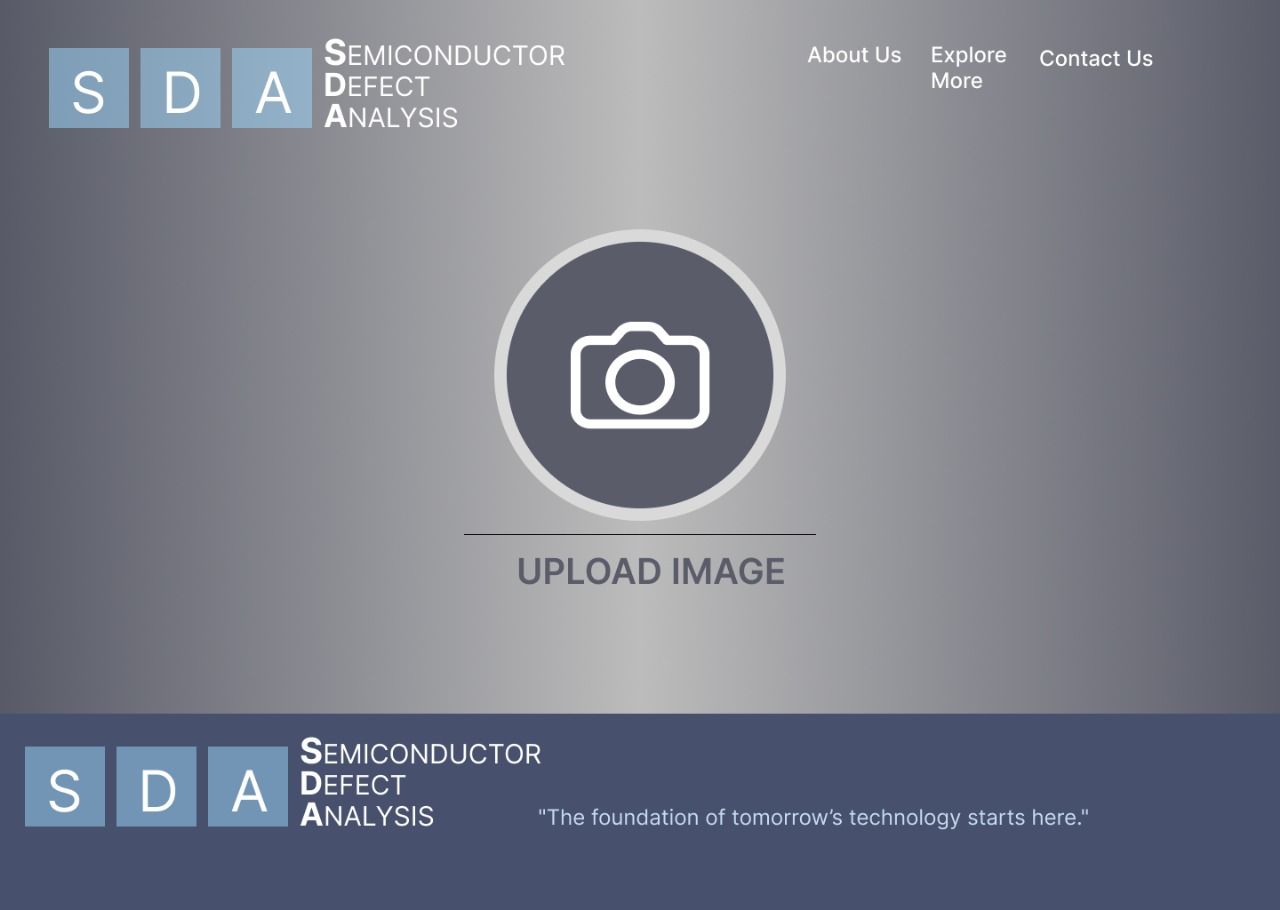
\includegraphics[width=9cm, height=7cm]{root/Website_homepage.jpg} % 1280x910
		\caption{Website Interface}
	\end{minipage}
	\hfill
	\begin{minipage}{0.4\textwidth}
		\centering
		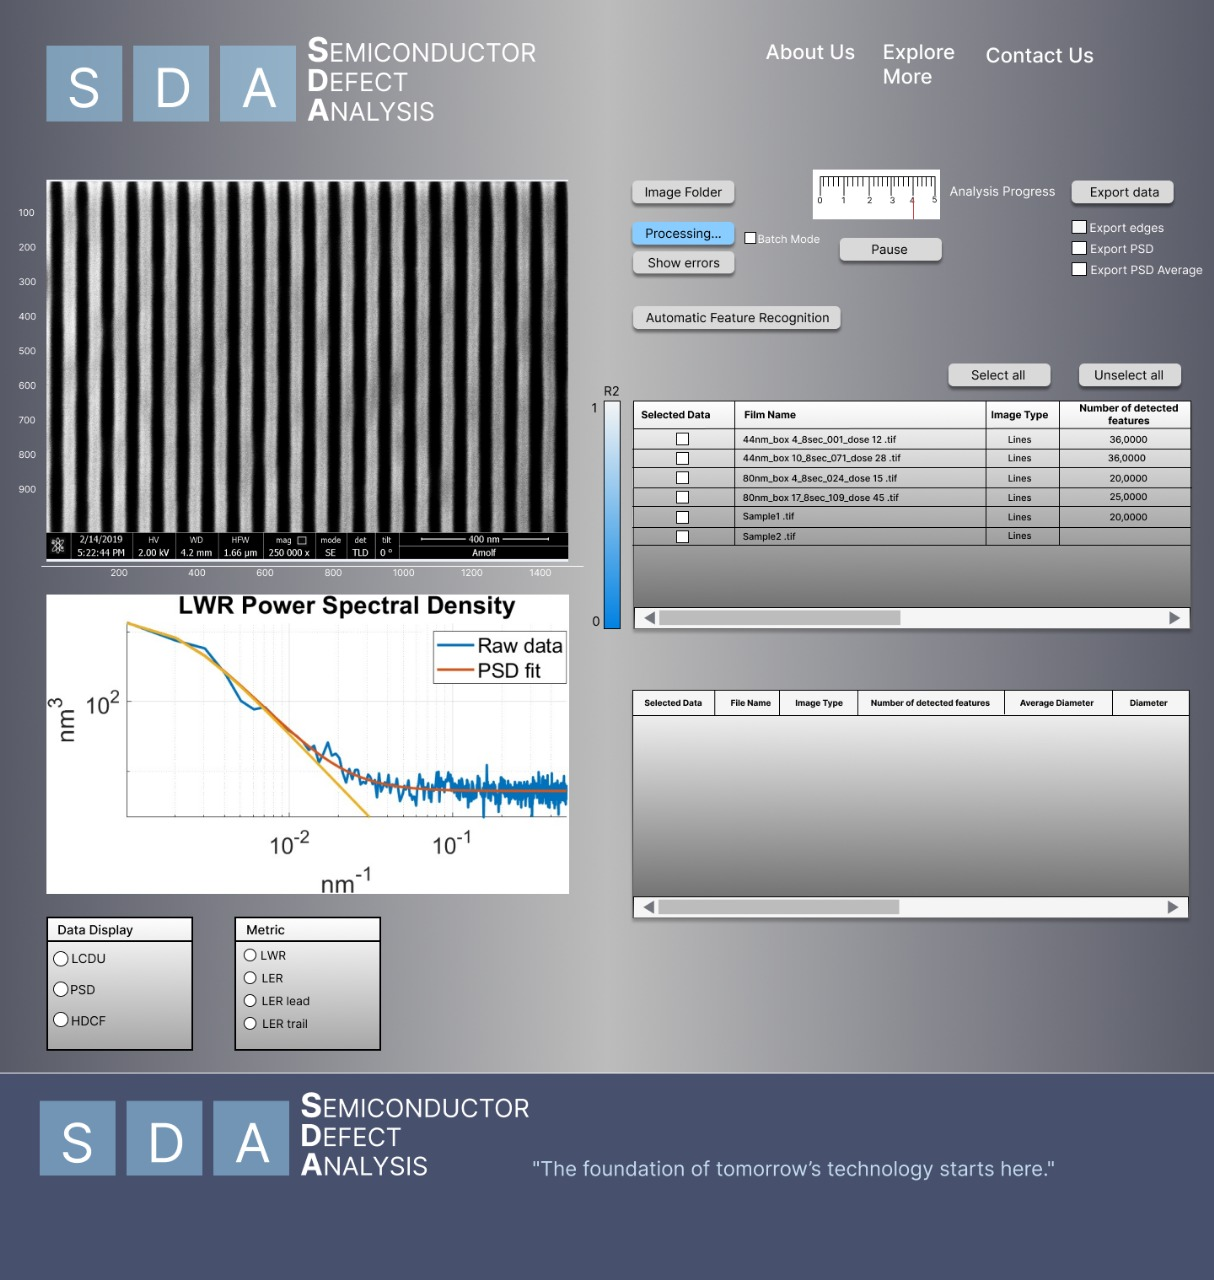
\includegraphics[width=9cm, height=7cm]{root/after_detects.jpg} % 1214x1280
		\caption{SEM Images Analysis}
	\end{minipage}
	
	\vspace{0.5cm} % Space between rows
	
	\begin{minipage}{0.7\textwidth}
		\centering
		
\includegraphics[width=7cm, height=13cm]{root/info.jpg} % 580x1280
		\caption{Website Landing Page}
	\end{minipage}
	
\end{figure}

% Restore the normal margins for the rest of the document
\restoregeometry

\section{Bill of Materials}
\vspace{0.5cm}
\renewcommand{\arraystretch}{2} % Adjust row height
\centering
\begin{tabular}{|c|c|c|c|}
	\hline
	Item Name & Quantity & Cost (in \scalebox{0.7}{\faRupeeSign}) & Vendor \\
	\hline
	Website Domain name & 1 & \scalebox{0.7}{\faRupeeSign} 8000 & Namecheap \\
	\hline
	Webhosting & 1 & \scalebox{0.7}{\faRupeeSign} 16000 & Render \\
	\hline
\end{tabular}

\vspace{0.25cm}
\begin{flushleft}
	Total Cost of the Items: \scalebox{0.7}{\faRupeeSign} 24000
\end{flushleft}

\vspace{1cm}
\begin{figure}[h]
	\hfill
	
\includegraphics[width=9.7cm, height=6cm]{root/newsign.png}
\end{figure}

\label{endOfDoc}
\end{document}
